\documentclass{article}
\usepackage[utf8]{inputenc}
\usepackage{geometry}
\usepackage{amsmath}
\usepackage{physics}
\usepackage{graphicx}
\usepackage{textcomp}
\usepackage{hyperref}
\geometry{legalpaper, portrait, margin = 0.5in}
\rmfamily

\title{CSE 390 HW4}
\author{David S. Li (SBUID: 110328771)}
\date{December 10, 2018}

\begin{document}

\maketitle

\section{ACF and PACF Plots}
\par\noindent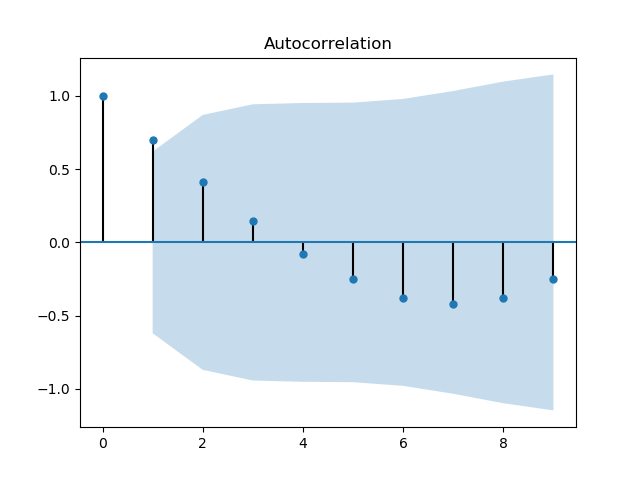
\includegraphics{Figure_1.png}
\par\noindent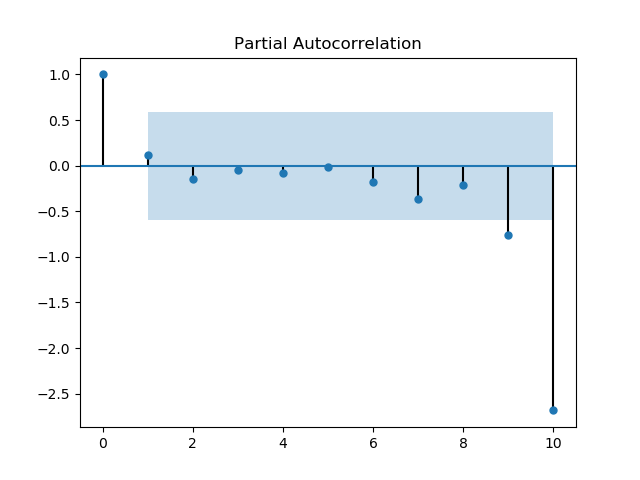
\includegraphics{Figure_2.png}

\section{$AR(p)$ model}

\par\noindent\Large $r_{t} = 0.003385 + 0.148171r_{t - 1} - 0.061258r_{t - 2} - 0.003243r_{t - 3} - 0.001238r_{t - 4} + 0.048897r_{t - 5}$

\par\noindent\Large Our max order, $p$ will be 5.  After that, the PACF graph starts to depart from the normal pattern, with values with an absolute value greater than 0.5.  The value of $p = 5$ is the closest the graph will get to 0.
\section{$MA(q)$ model}

\par\noindent\Large $r_{t} = 0.00457058 + a_{t} - 0.14824403a_{t - 1} + 0.06048652a_{t - 2} + 0.00254155a_{t - 3} + 0.0010591a_{t - 4}$

\par\noindent\Large Our max order, $q$ will be 4.  That is the closest that the absolute value of something on the ACF graph will get to 0.  After that, the values gradually start to expand out again.

\section{Justification for value of $p$ and $q$}

\par\noindent\Large The values of $p$ and $q$ are 5 and 4 respectively.  In the PACF and ACF graphs, at that point, the absolute value of the index to 0 comes closest to reaching 0 before the graph starts to expand out again.  In the evaluated parameters, where a maximum lag of 10 was given, the parameters themselves showed very similar trends, with the expansion starting at indices not too far from the specified $p$ and $q$ values.

\par\noindent\Large 
\end{document}
